\begin{frame}\begin{center}
\LARGE\textbf{Mincer returns}
\end{center}\end{frame}
%-------------------------------------------------------------------------------
%-------------------------------------------------------------------------------
\begin{frame}
\textbf{Mincer Equation}\\
\begin{align*}
\ln{Y(s, x)} = \alpha + \rho_s s + \beta_0 x + \beta_1 x^2 + \epsilon\\
\end{align*}
$\Rightarrow$ How to interpret the \textit{Mincer Coefficient} $\rho_s$?
\end{frame}
%-------------------------------------------------------------------------------
%-------------------------------------------------------------------------------
\begin{frame}\textbf{Conceptual Frameworks}\vspace{0.3cm}
\begin{itemize}\setlength\itemsep{1em}
\item compensating differences
\item accounting-identity
\end{itemize}
\end{frame}
%-------------------------------------------------------------------------------
%-------------------------------------------------------------------------------
\begin{frame}\begin{center}
\LARGE\textit{Compensating Differences Model}
\end{center}\end{frame}
%-------------------------------------------------------------------------------
%-------------------------------------------------------------------------------
\begin{frame}
Let $Y(s)$ represent the annual earnings of an individual with $s$ years of education, assumed to be constant over his lifetime. Let $r$ be an externally determined interest rate and $T$ the length of working life, assumed not to depend on $s$. The present value of earnings associated with schooling level $s$ is

\begin{align*}
V(s) = Y(s)\int_s^T e^{-rt} dt = \frac{Y(s)}{r}(e^{-rs} - e^{-rT}).
\end{align*}
\end{frame}
%-------------------------------------------------------------------------------
%-------------------------------------------------------------------------------
\begin{frame}
\begin{figure}[htp]\centering
\caption{Earnings}\scalebox{0.35}
{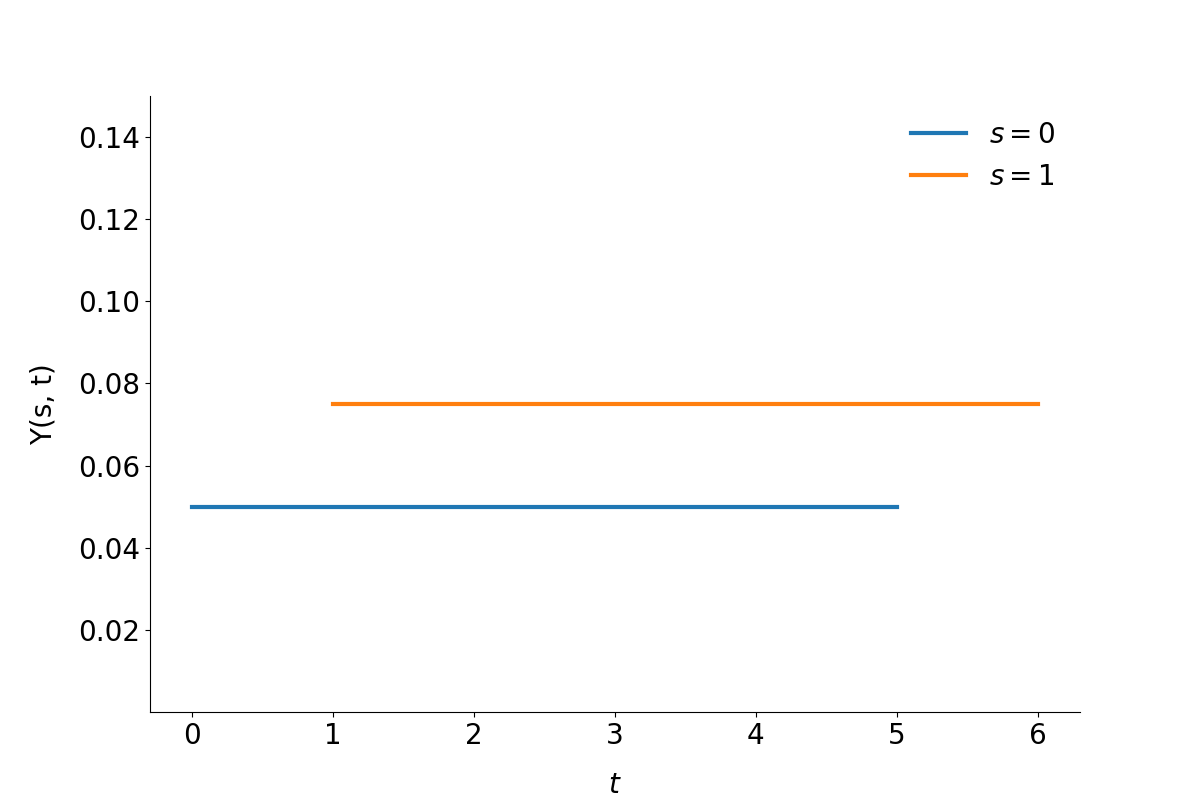
\includegraphics{fig-model-mincer-return-earnings}}
\end{figure}
\end{frame}
%-------------------------------------------------------------------------------
%-------------------------------------------------------------------------------
\begin{frame}
\begin{figure}[htp]\centering
\caption{Value}\scalebox{0.35}
{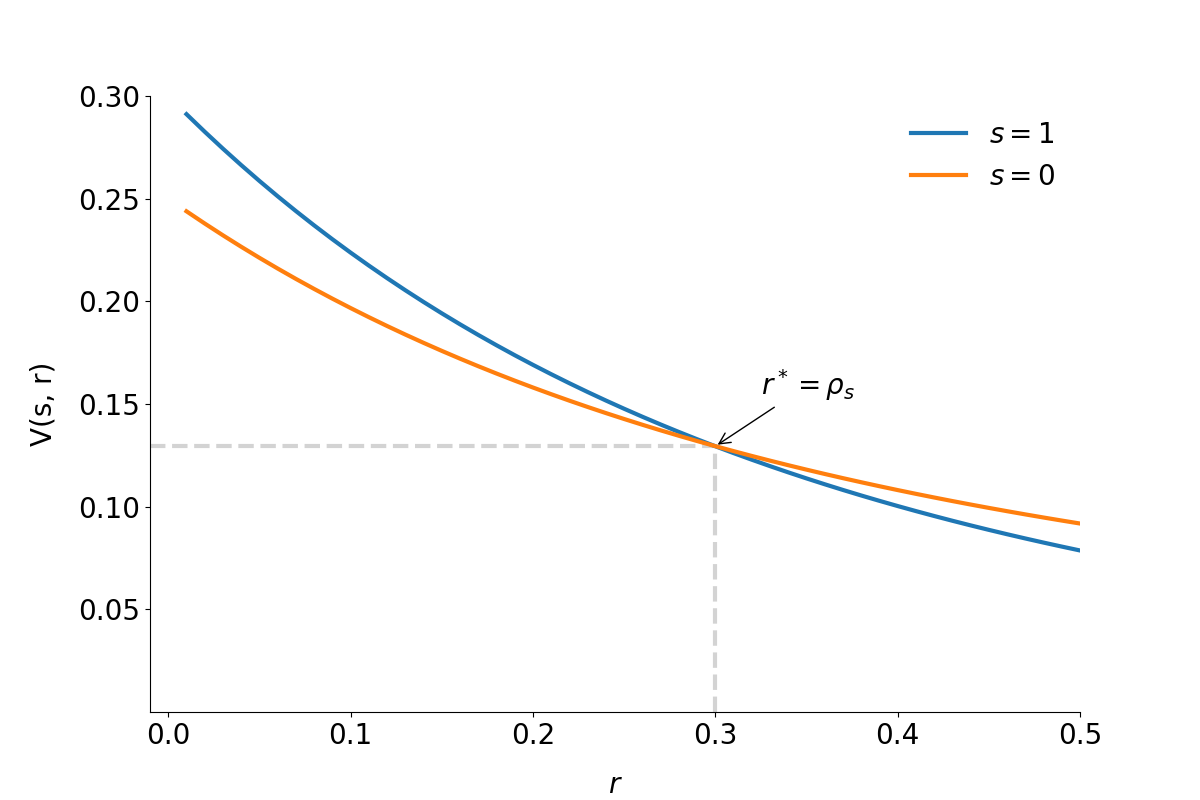
\includegraphics{fig-model-mincer-return-value}}
\end{figure}
\end{frame}
%-------------------------------------------------------------------------------
%-------------------------------------------------------------------------------
\begin{frame}

Equilibrium across heterogeneous schooling levels requires that individuals be indifferent between schooling choices, with allocations being driven by demand conditions.
Equating earnings streams across schooling levels and taking logs yields
\begin{align*}
\ln{Y(s)} = \ln{Y(0)} + r s + \ln{\left(\frac{1 -e^{-rs}}{1 - e^{-r(T - s)}}\right)}. \\
\end{align*}

$\Rightarrow$ $\rho_s$ equals the market interest rate and the internal rate of return to schooling by construction.
\end{frame}
%-------------------------------------------------------------------------------
%-------------------------------------------------------------------------------
\begin{frame}\textbf{Model features}\vspace{0.3cm}
\begin{itemize}\setlength\itemsep{1em}
\item identical abilities and opportunities
\item no credit constraints
\item perfect certainty
\item no direct cost of schooling
\item no nonpecuniary benefits of school and work
\end{itemize}
\end{frame}
%-------------------------------------------------------------------------------
%-------------------------------------------------------------------------------
\begin{frame}\begin{center}
    \LARGE\textit{Accounting-Identity Model}
\end{center}\end{frame}
%-------------------------------------------------------------------------------
%-------------------------------------------------------------------------------
\begin{frame}\textbf{Model ingredients}
\begin{align*}\begin{array}{ll}
P_t & \text{potential earnings at $t$} \\
C_t = k_t P_t & \text{investment cost of training at $t$} \\
\rho_t & \text{average return to investment at $t$}
\end{array}\end{align*}
\end{frame}
%-------------------------------------------------------------------------------
%-------------------------------------------------------------------------------
\begin{frame}
\begin{align*}
P_t & \equiv P_{t - 1} (1 + k_{t - 1} \rho_{t - 1}) \equiv \prod^{t - 1}_{j= 0} (1 + \rho_jk_j)P_0 \\
\end{align*}
\end{frame}
%-------------------------------------------------------------------------------
%-------------------------------------------------------------------------------
\begin{frame}
Formal schooling is defined as years spent in full-time investment $(k_t = 1)$, which is assumed to take place at the beginning of life and to yield a rate of return $\rho_s$ that is constant across all years of schooling.

\begin{align*}
\ln{P_t} & \equiv \ln{P_0}  + s \ln{(1 + \rho_s)} + \sum^{t-1}_{j=s} \ln{(1 + \rho_0 k_j)} \\
& \approx  \ln{P_0} + s \rho_s + \rho_0 \sum^{t - 1}_{j=s} k_j
\end{align*}
\end{frame}
%-------------------------------------------------------------------------------
%-------------------------------------------------------------------------------
\begin{frame}
\citeA{Mincer.1974} assumes a linearly declining rate of post-school investment:
\begin{align*}
k_{s + x} = \kappa\left( 1 - x/T\right), \text{where}\; x = t - s
\end{align*}
\end{frame}
%-------------------------------------------------------------------------------
%-------------------------------------------------------------------------------
\begin{frame}
\begin{figure}[htp]\centering
\caption{Post-School Investment}
\scalebox{0.30}{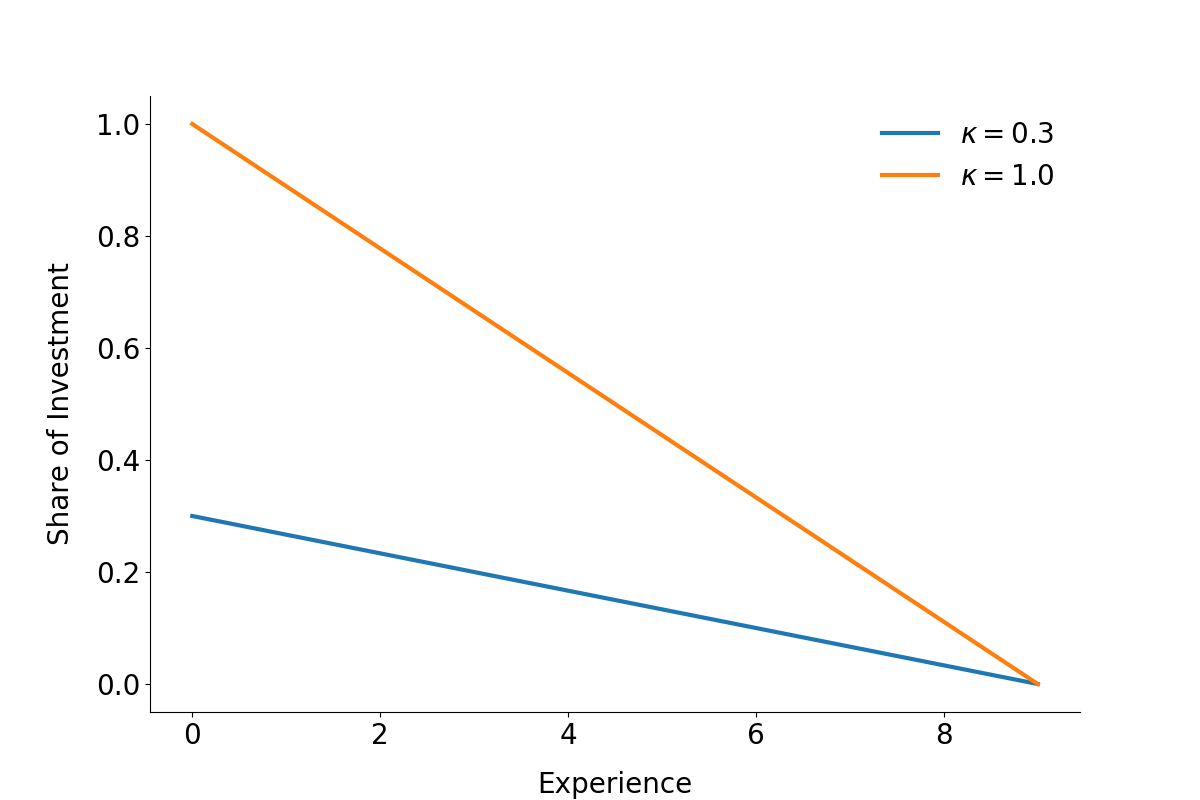
\includegraphics{fig-model-mincer-post-school}}
\end{figure}
\end{frame}
%-------------------------------------------------------------------------------
%-------------------------------------------------------------------------------
\begin{frame}
The derivations draws on the following results for arithmetic series \cite{Chapman.2018}.
\begin{align*}
\sum^n_{i = 0} i = \sum^n_{i = 1} i = \frac{n(n + 1)}{2}
\end{align*}
\end{frame}
%-------------------------------------------------------------------------------
%-------------------------------------------------------------------------------
\begin{frame}

 \begin{align*}
 \ln{P_{x + s}}  \approx \ln{P_0} + s\rho_s + \underbrace{\left(\rho_0 \kappa + \frac{\rho_0\kappa}{2T}\right)x - \frac{\rho_0\kappa}{2T} x^2}_{(1)} \\
\end{align*}

You can derive $(1)$ using the previous results.

\end{frame}
%-------------------------------------------------------------------------------
%-------------------------------------------------------------------------------
\begin{frame}
Accounting for the difference in potential and observed earnings:
\begin{align*}
\ln{Y(s, x)} & \approx \ln{P_{x + s}} - \kappa\left(1 - x/T\right) \\
            & = [\ln{P_0} - \kappa] + \rho_s s + \left(\rho_0\kappa + \frac{\rho_0\kappa}{2T} + \frac{\kappa}{T}\right) x - \frac{\rho_0\kappa}{2T}x^2
\end{align*}
$\Rightarrow$ $\rho_s$ is the average earnings increase with schooling
\end{frame}
%-------------------------------------------------------------------------------
%-------------------------------------------------------------------------------
\begin{frame}
\textbf{Standard Mincer Equation}
\begin{align*}
\ln Y(s, x) = \alpha + \rho_s s + \beta_0 x + \beta_1 x^2,
\end{align*}
where
\begin{align*}
\alpha & =\ln{P_0} - \kappa \\
\beta_0 & = \left(\rho_0\kappa + \frac{\rho_0\kappa}{2T} + \frac{\kappa}{T}\right) \\
\beta_1 & = -\frac{\rho_0\kappa}{2T}\\
\end{align*}

What about heterogeneous returns?

\end{frame}
%-------------------------------------------------------------------------------
%-------------------------------------------------------------------------------
\begin{frame}
\textbf{Random Coefficient Version}
\begin{align*}
\ln{Y(s_i, x_i)} = \alpha_{i} + \rho_{si} s_i + \beta_{0i} x_i + \beta_{1i} x_i^2
\end{align*}
and let
\begin{align*}
\bar{\alpha} = \E[\alpha_i] &\qquad \bar{\rho}_s = \E[\rho_{si}]\\
\bar{\beta}_0 = \E[\beta_{0i}]&\qquad \bar{\beta}_1 = \E[\beta_{1i}]
\end{align*}
\end{frame}
%-------------------------------------------------------------------------------
%-------------------------------------------------------------------------------
\begin{frame}
Dropping individual subscripts ...

\begin{align*}
\ln{Y(s, x)} & = \bar{\alpha} + \bar{\rho}_s s + \bar{\beta}_{0} x + \bar{\beta}_{1} x^2 \\
                & + \underbrace{[(\alpha - \bar{\alpha}) + (\rho_s - \bar{\rho}_s) s + (\beta_0 - \bar{\beta}_0)x + (\beta_1 - \bar{\beta}_1)x^2 ]}_{\epsilon}\\
\end{align*}
$\Rightarrow$ If the schooling decision is determined by individual returns, then we are back in the case of a correlated random coefficient model \cite{Heckman.2006d}.
\end{frame}
%-------------------------------------------------------------------------------
%-------------------------------------------------------------------------------
\begin{frame}[plain]

\begin{center}
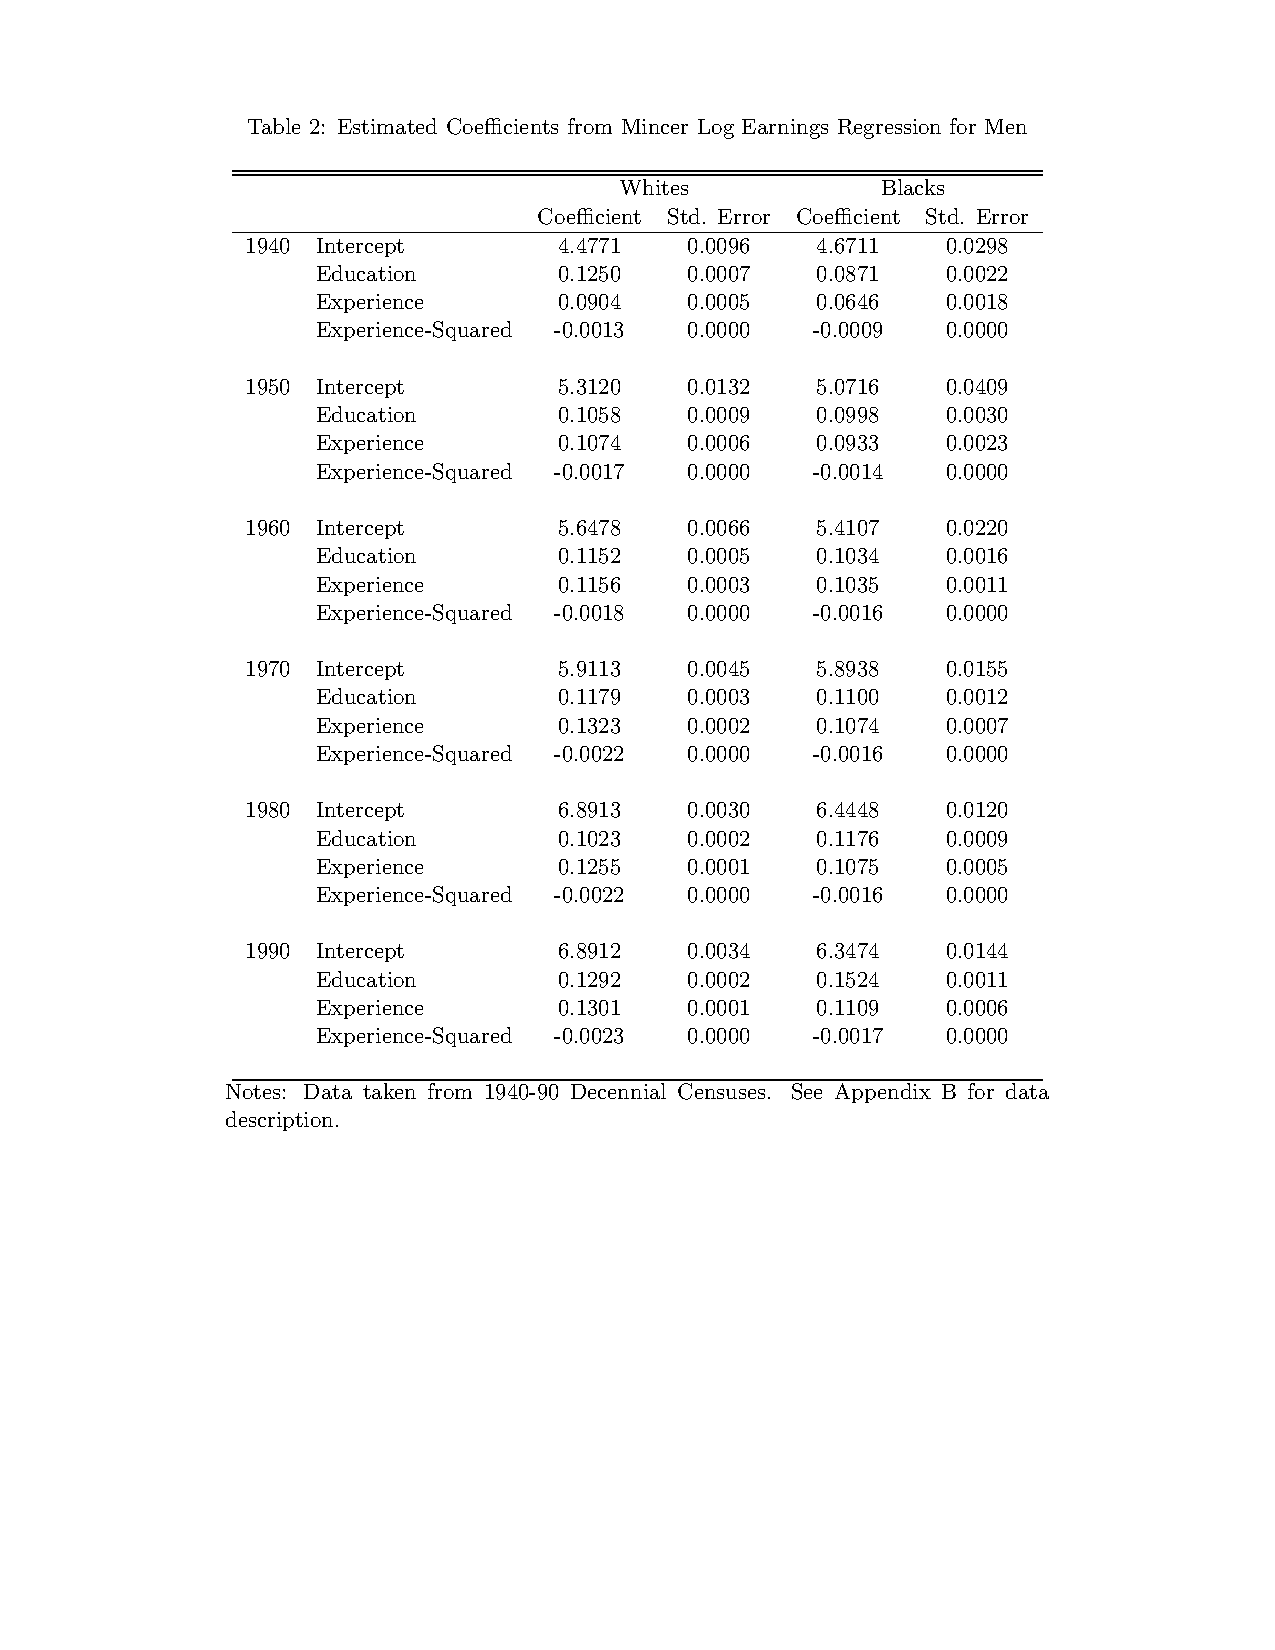
\includegraphics[width=.65\columnwidth]{fig-mincer-regressions}
\end{center}

\end{frame}
%-------------------------------------------------------------------------------
%-------------------------------------------------------------------------------
\begin{frame}
We can analyze this model in a Jupyter Noteboook. Visit
\begin{center}
\url{http://bit.ly/2kAtcyg}
\end{center}
for the implementation.
\end{frame}
%-------------------------------------------------------------------------------
%-------------------------------------------------------------------------------
\begin{frame}\begin{center}
\LARGE\textit{Implications}
\end{center}\end{frame}
%-------------------------------------------------------------------------------
%-------------------------------------------------------------------------------
\begin{frame}
\begin{itemize}
\item Log-earnings profiles are parallel across schooling levels.
\begin{align*}
\frac{\partial \ln{Y(s, x)}}{\partial s \partial x} = 0
\end{align*}
\item Log-earnings age profiles diverge with age across schooling levels.
\begin{align*}
\frac{\partial \ln{Y(s, x)}}{\partial s \partial t} = \frac{\rho_0\kappa}{T} > 0
\end{align*}
\end{itemize}
\end{frame}
%-------------------------------------------------------------------------------
%-------------------------------------------------------------------------------
\begin{frame}
\begin{figure}[htp]\centering
\caption{Experience profiles}\scalebox{0.3}{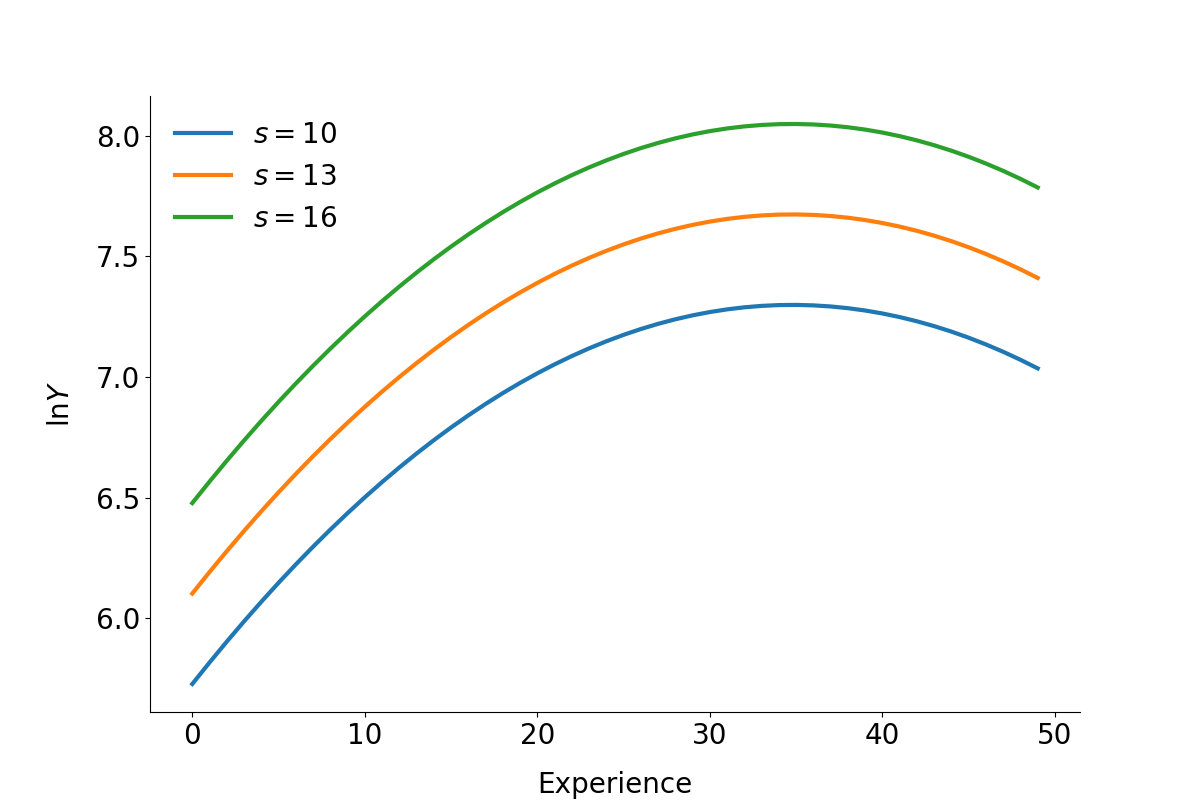
\includegraphics{fig-model-mincer-experience}}
\end{figure}
\end{frame}
%-------------------------------------------------------------------------------
%-------------------------------------------------------------------------------
\begin{frame}
\begin{figure}[htp]\centering
\caption{Age profiles}\scalebox{0.3}{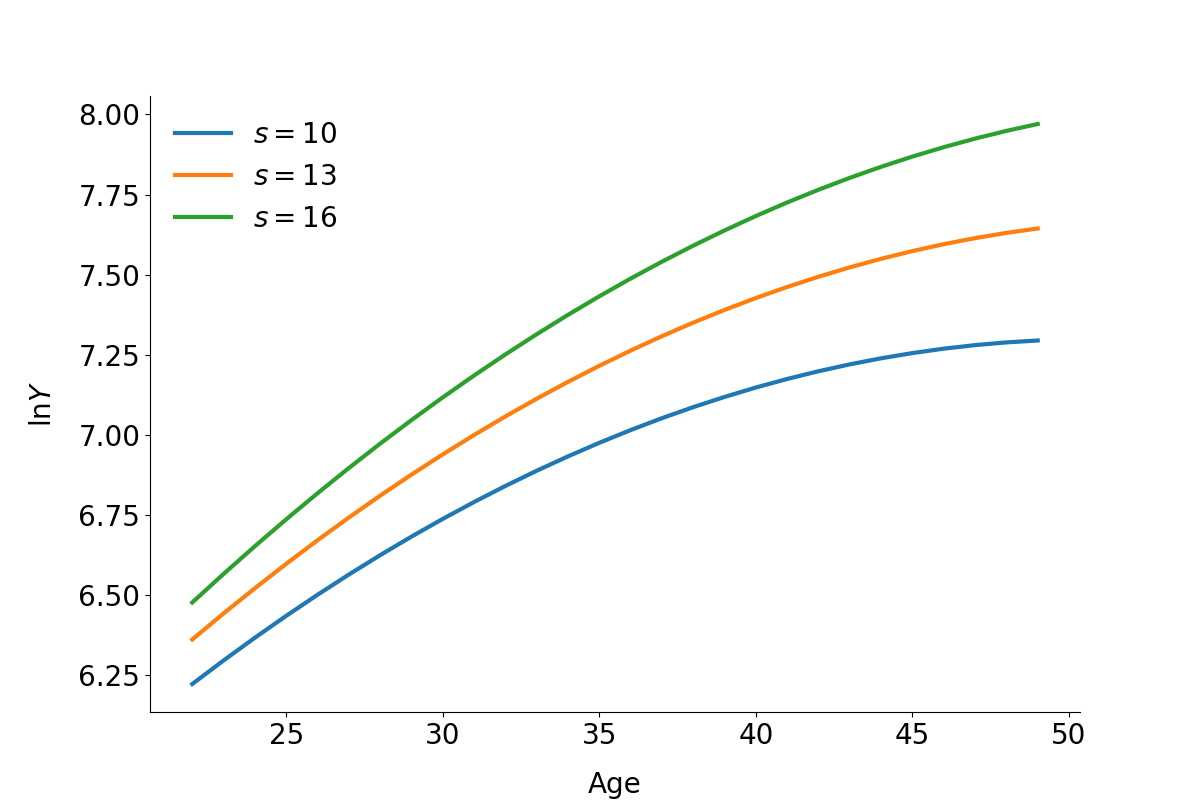
\includegraphics{fig-model-mincer-age}}
\end{figure}
\end{frame}
%-------------------------------------------------------------------------------
%-------------------------------------------------------------------------------
\begin{frame}
\begin{itemize}
\item The variance of earnings over the life cycle has a U-shaped pattern.
\end{itemize}
\end{frame}
%-------------------------------------------------------------------------------
%-------------------------------------------------------------------------------
\begin{frame}\textbf{Derivation for minimizing variance}\vspace{0.3cm}
	\begin{align*}
	\ln{Y(s,x)} & = \ln{P_{s+x}} + \ln{(1 - k_{s+x})} \\
	& \approx \ln{P_s} + \rho_0 \sum^{x - 1}_{j=0} k_{s+j} - k_{s+x}
	\end{align*}

	Further, using the assumption of linearly declining investment yields

	\begin{align*}
	\ln{Y(s,x)} \approx \ln{P_s} + \kappa \left(\rho_0 \sum^{x - 1}_{j=0} (1 - j/T) - (1 - x/T)\right) \\
	\end{align*}
\end{frame}
%-------------------------------------------------------------------------------
%-------------------------------------------------------------------------------
\begin{frame}
	Assuming only initial earnings potential $P_s$ and investment levels $\kappa$ vary in the population, the variance of log earnings is given by

	\begin{align*}
	\var(\ln{Y(s,x)}) & = \var(\ln{P_s}) \\
	& + \left(\rho_0 \sum^{x - 1}_{j=0} (1 - j/T) - (1 - x/T)\right)^2 \var(\kappa) \\
	& + 2\left(\rho_0 \sum^{x - 1}_{j=0} (1 - j/T) - (1 - x/T)\right) \cov(\ln{P_s},k).
	\end{align*}
\end{frame}
%-------------------------------------------------------------------------------
%-------------------------------------------------------------------------------
\begin{frame}
	If $\kappa$ and $\ln{P_s}$ are uncorrelated, then earnings are minimized (and equal to $Var(\ln{P_s})$)
	when

	\begin{align*}
	\rho_0 \sum^{x - 1}_{j=0} (1 - j/T) = 1 - x/T, or \\
	\\
	\rho_0\left(x - \frac{x(x - 1)}{2T}\right) = (1 - x/T).
	\end{align*}
\end{frame}
%-------------------------------------------------------------------------------
%-------------------------------------------------------------------------------
\begin{frame}
	Clearly, $\lim_{T\to\infty} x^* = \frac{1}{\rho_0}$, so the variance minimizing age is $\frac{1}{\rho_0}$ when the work-life is long.
\end{frame}
%-------------------------------------------------------------------------------
%-------------------------------------------------------------------------------
\begin{frame}
\begin{figure}[htp]\centering
\caption{Variance profiles}\scalebox{0.3}{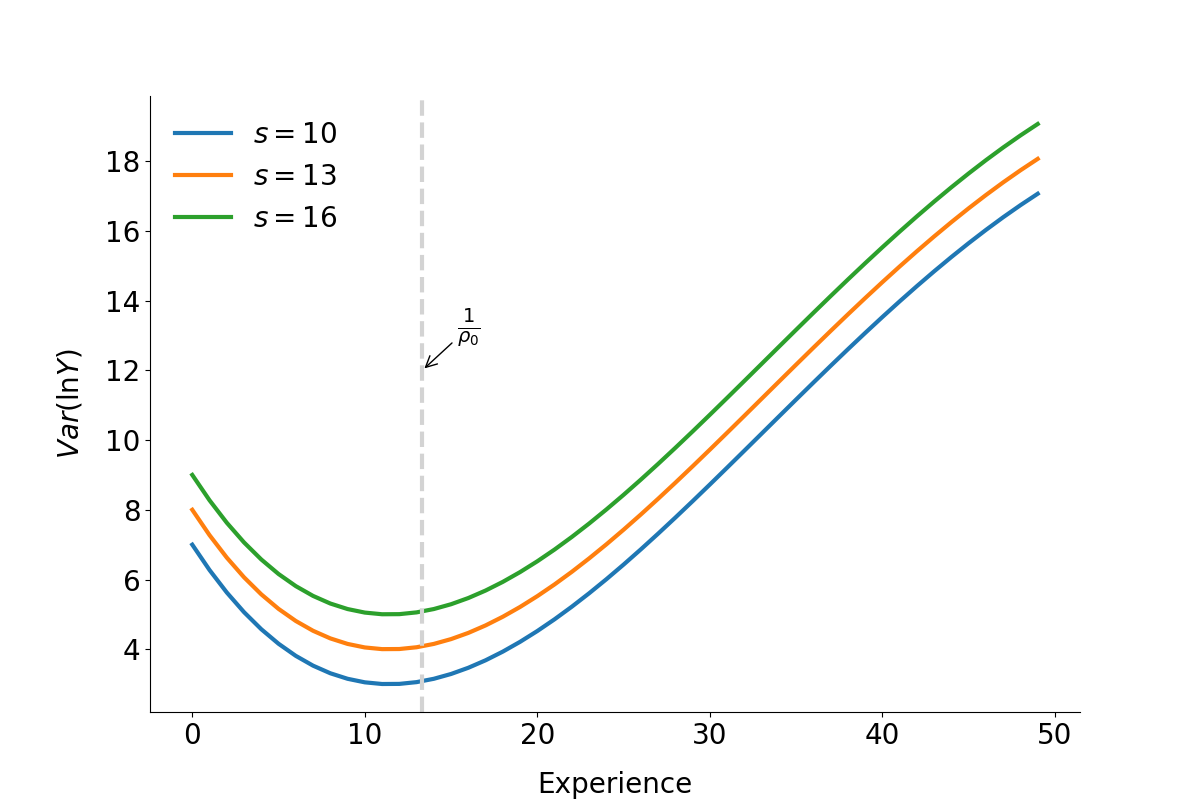
\includegraphics{fig-model-mincer-variance}}
\end{figure}
\end{frame}
%-------------------------------------------------------------------------------
%-------------------------------------------------------------------------------
\begin{frame}\begin{center}
\LARGE\textit{Empirical Evidence}
\end{center}\end{frame}
%-------------------------------------------------------------------------------
%-------------------------------------------------------------------------------
\begin{frame}[plain]
\begin{center}
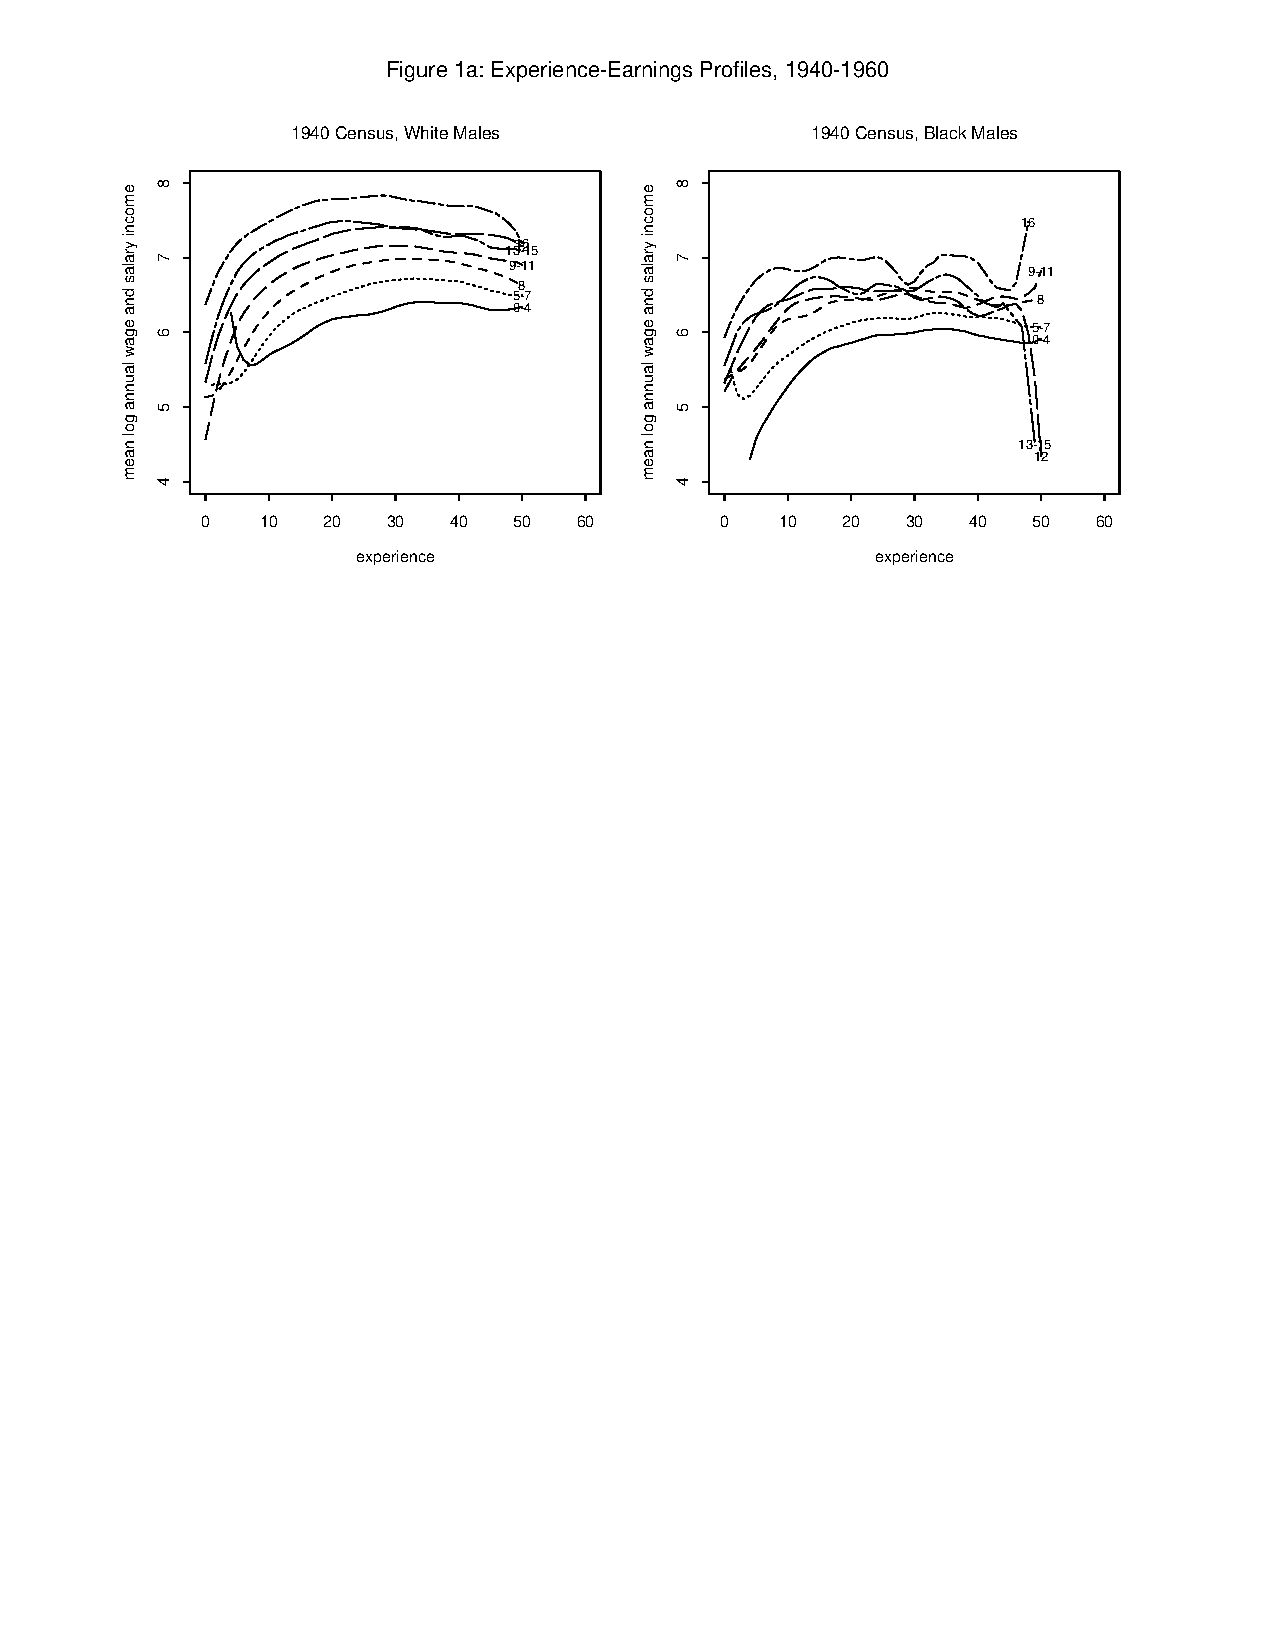
\includegraphics[width=.90\columnwidth]{fig-mincer-experience-1940}
\end{center}
\end{frame}
%-------------------------------------------------------------------------------
%-------------------------------------------------------------------------------
\begin{frame}[plain]
\begin{center}
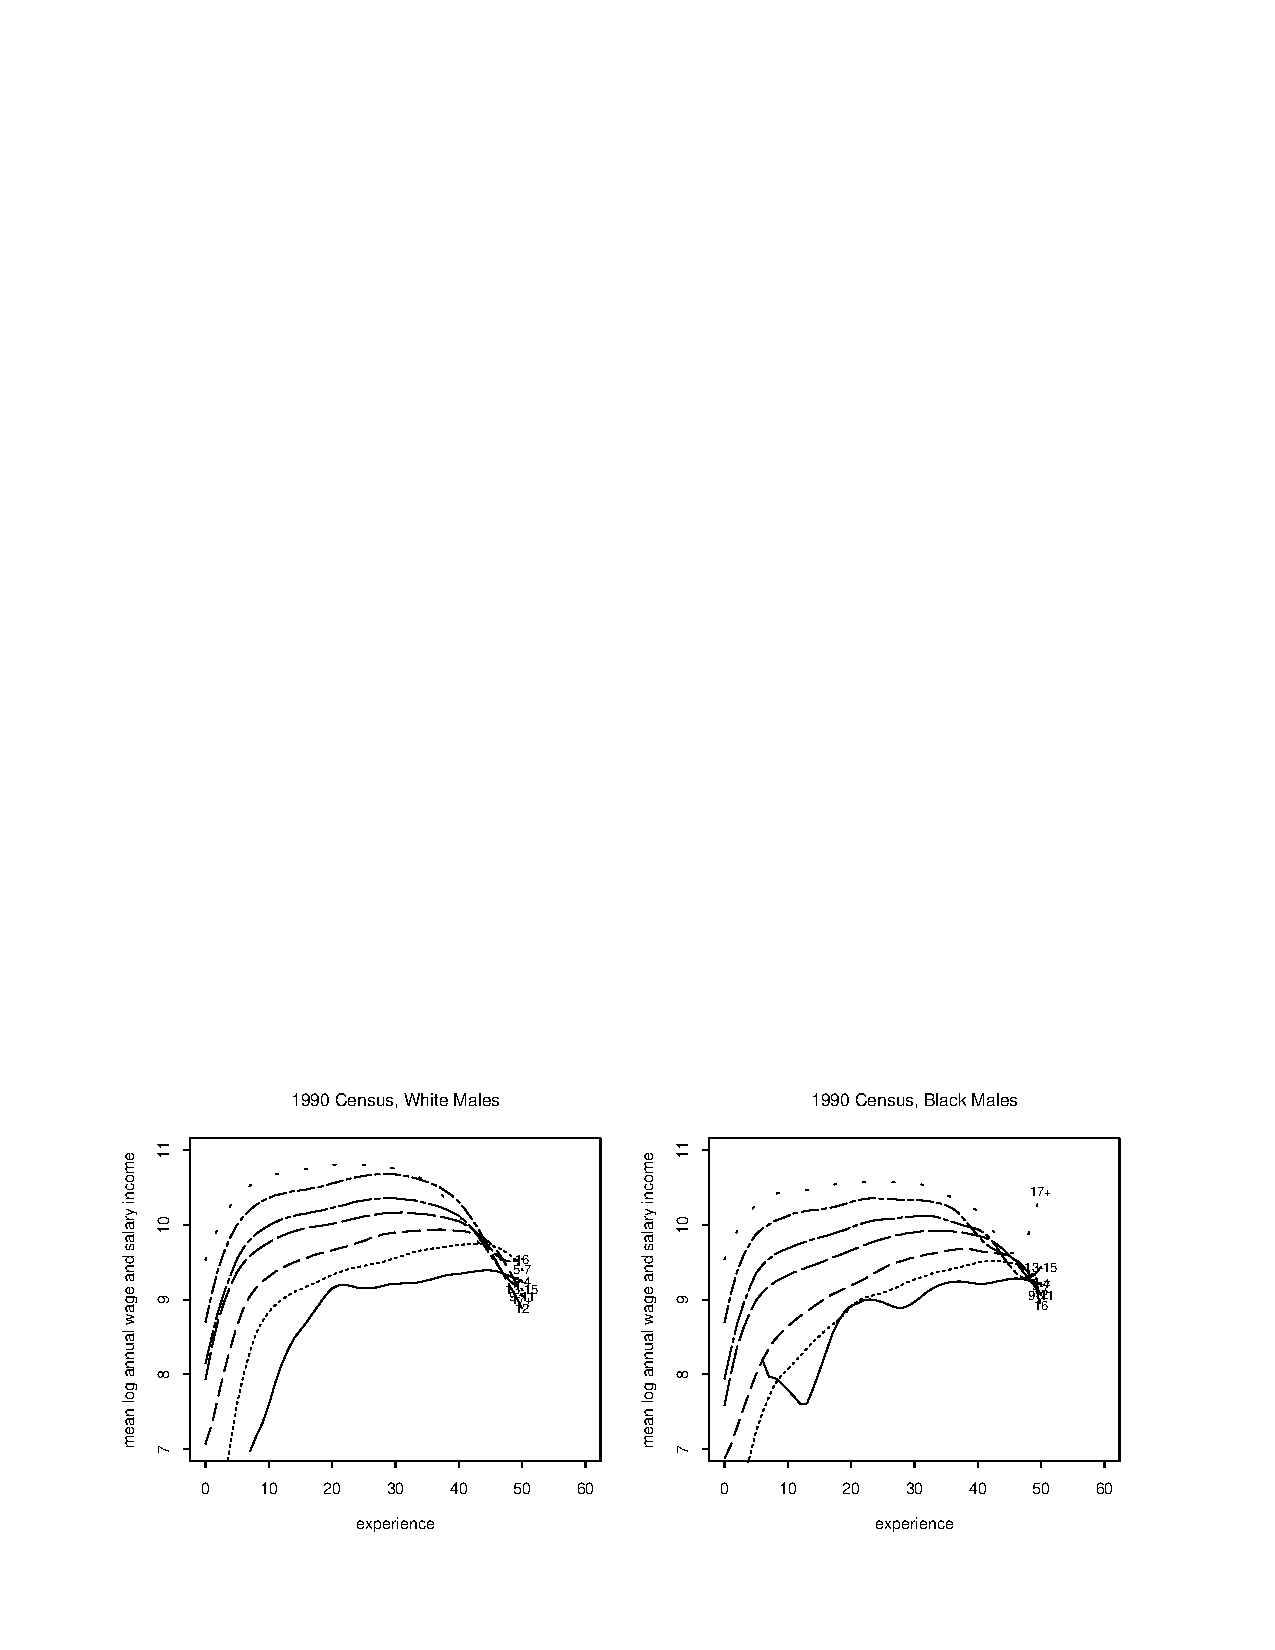
\includegraphics[width=.90\columnwidth]{fig-mincer-experience-1990}
\end{center}
\end{frame}
%-------------------------------------------------------------------------------
%-------------------------------------------------------------------------------
\begin{frame}[plain]
\begin{center}
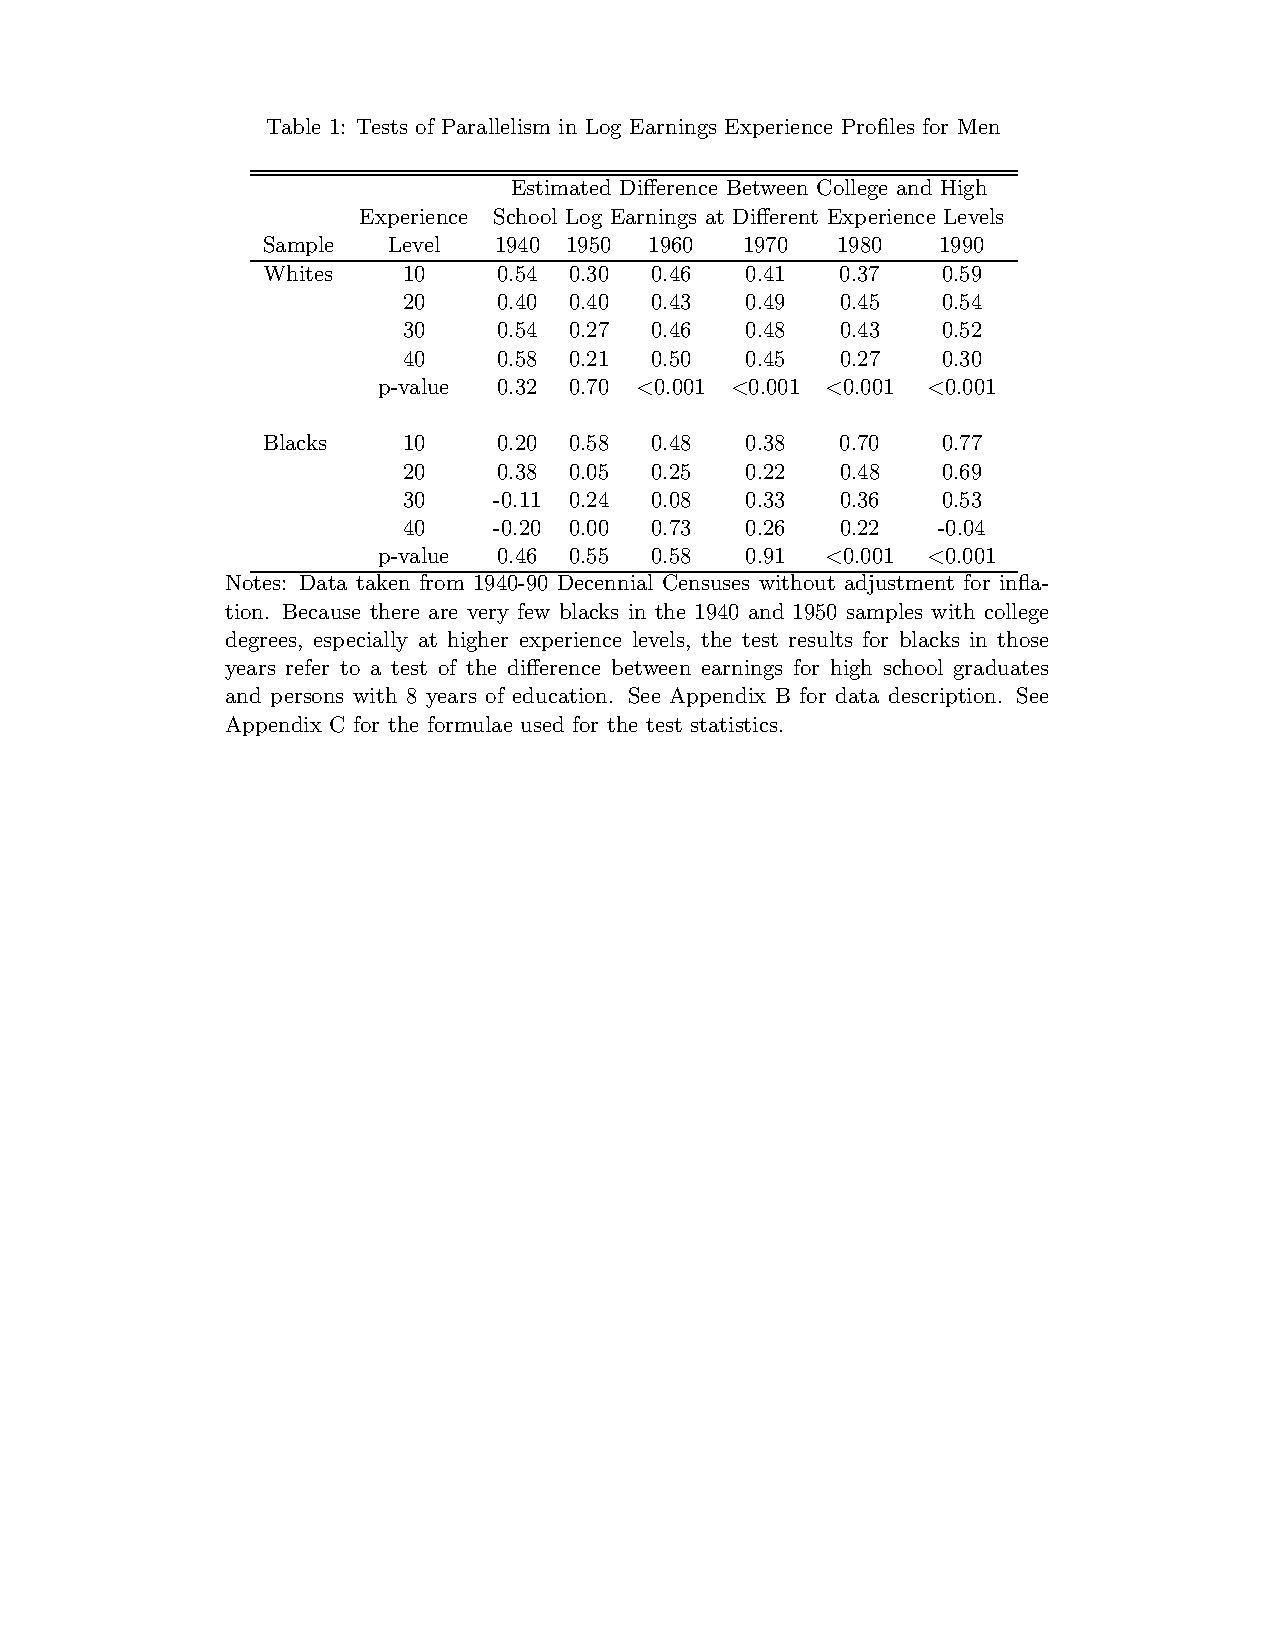
\includegraphics[width=.90\columnwidth]{fig-mincer-parallelism}
\end{center}
\end{frame}
%-------------------------------------------------------------------------------
%-------------------------------------------------------------------------------
\begin{frame}[plain]
\begin{center}
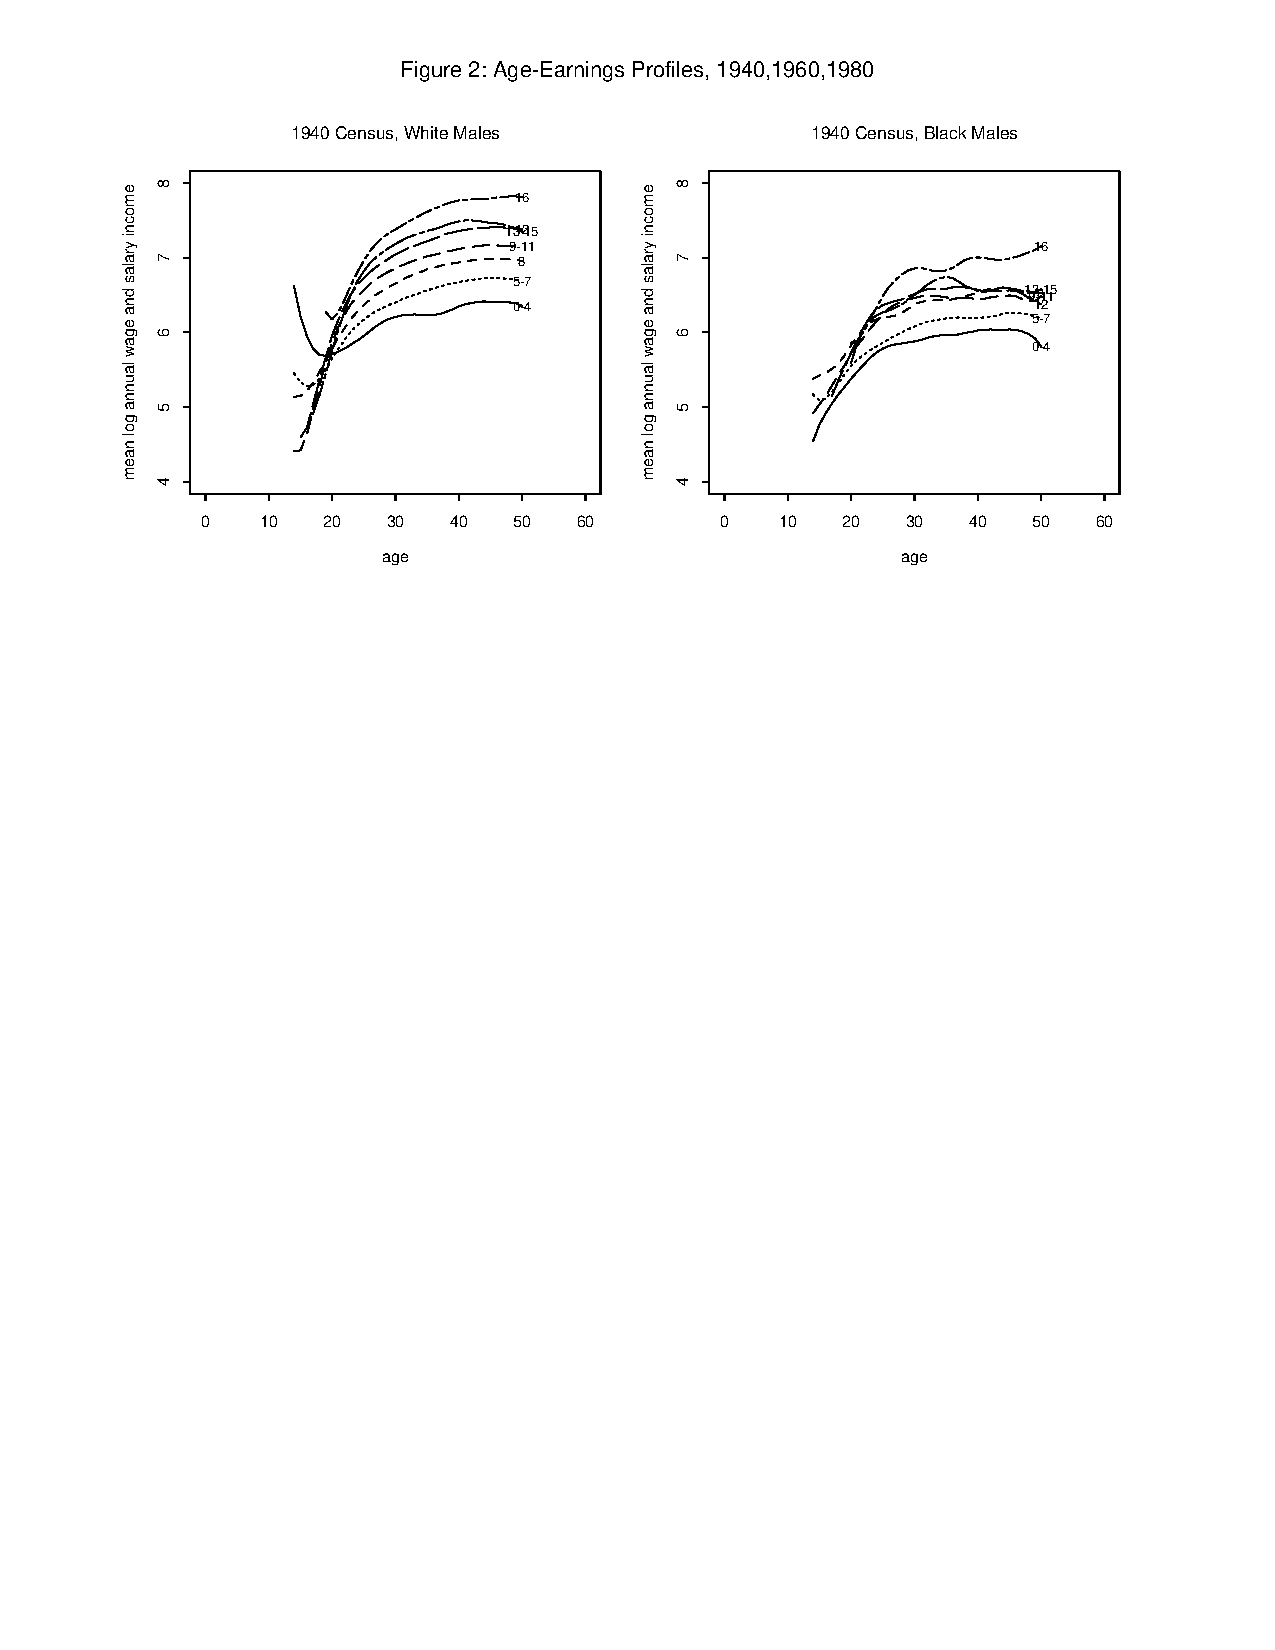
\includegraphics[width=.90\columnwidth]{fig-mincer-age-1940}
\end{center}
\end{frame}
%-------------------------------------------------------------------------------
%-------------------------------------------------------------------------------
\begin{frame}[plain]
\begin{center}
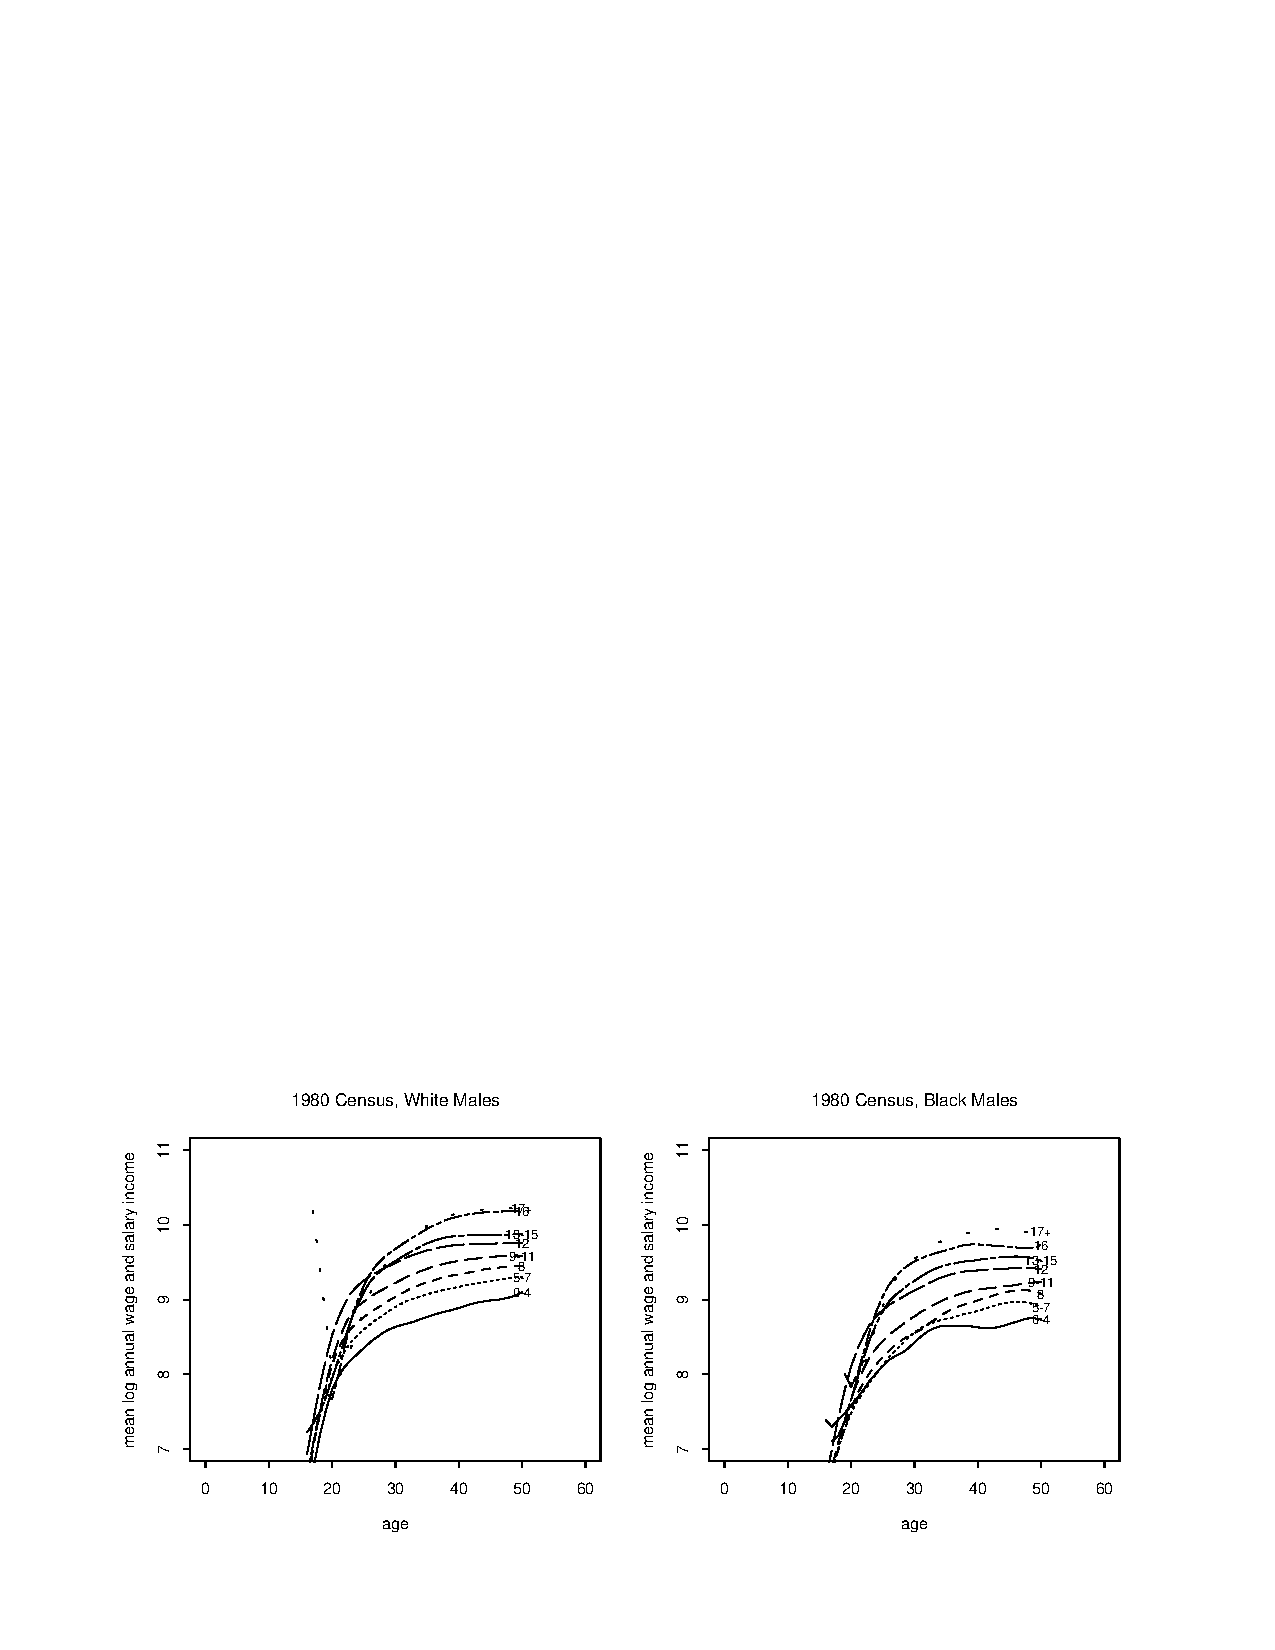
\includegraphics[width=.90\columnwidth]{fig-mincer-age-1980}
\end{center}
\end{frame}
%-------------------------------------------------------------------------------
%-------------------------------------------------------------------------------
\begin{frame}[plain]
\begin{center}
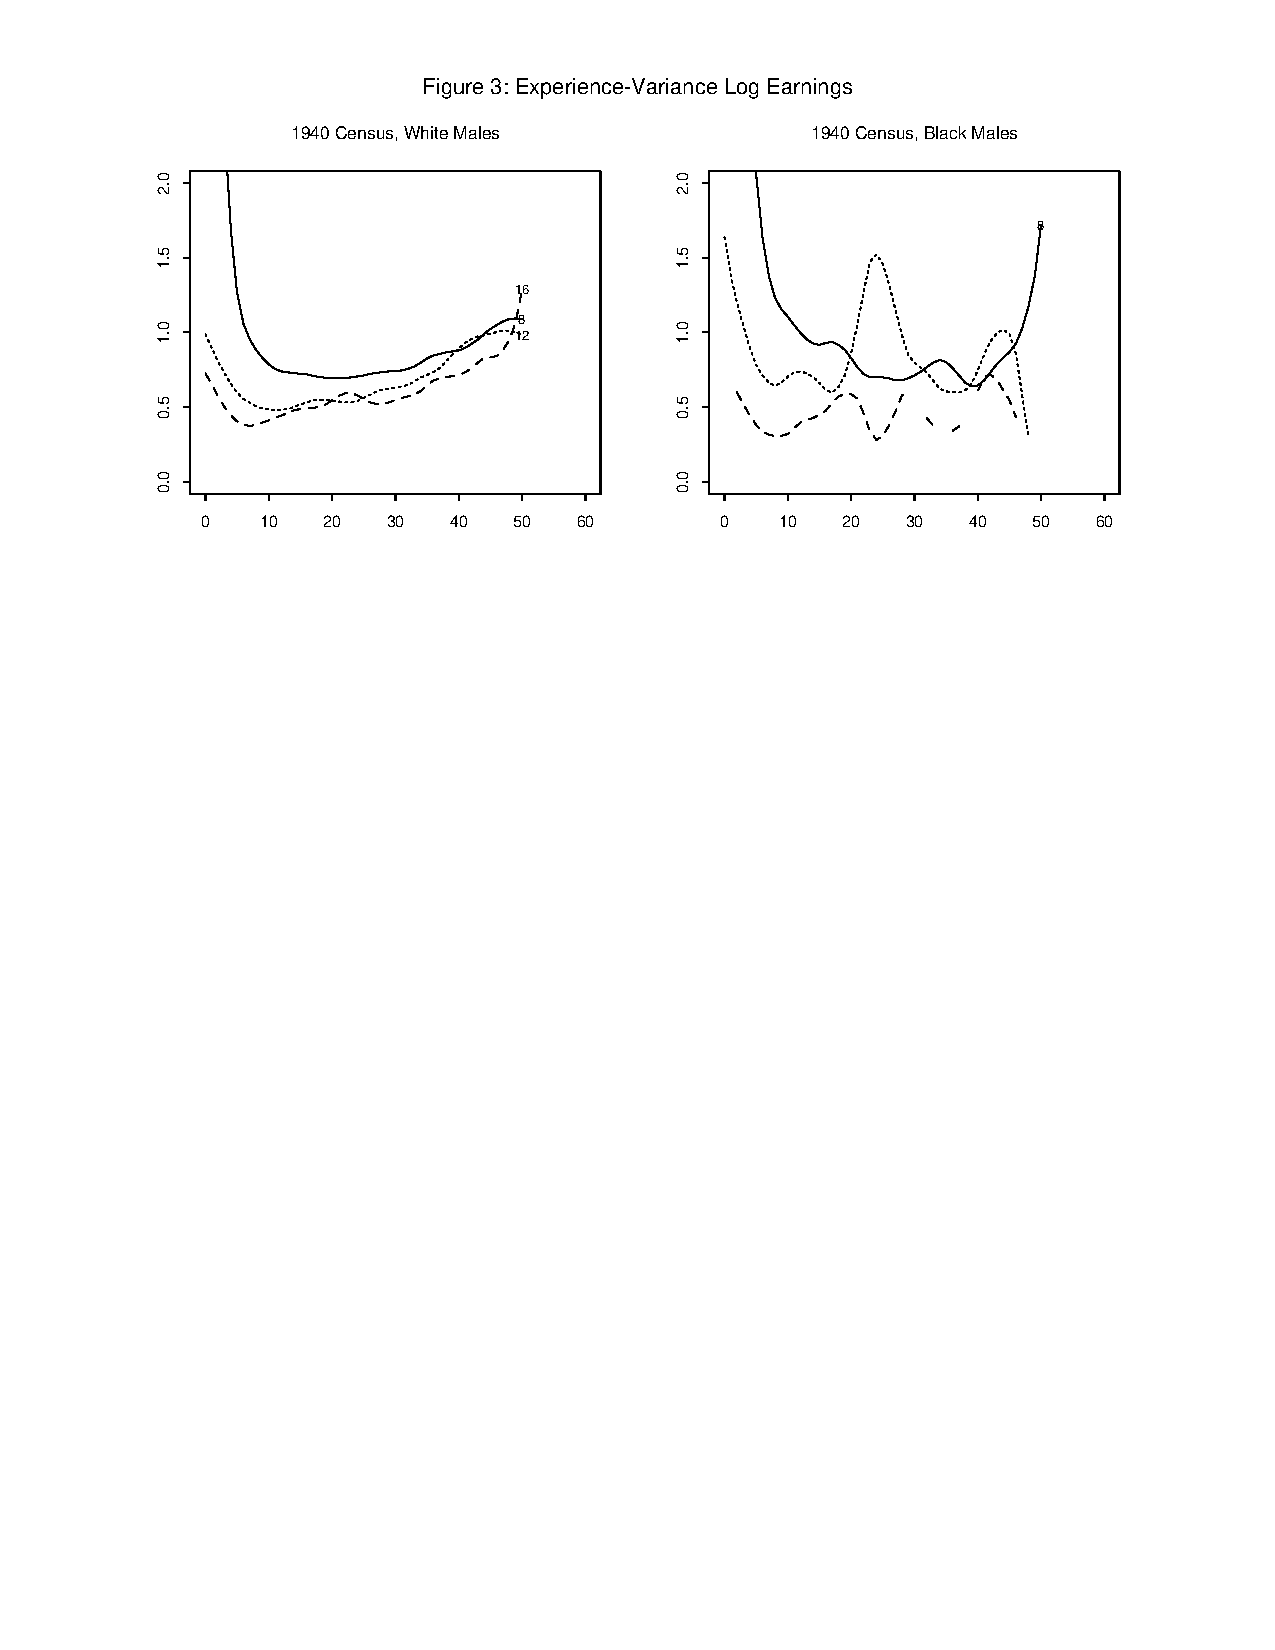
\includegraphics[width=.90\columnwidth]{fig-mincer-variance-1940}
\end{center}
\end{frame}
%-------------------------------------------------------------------------------
%-------------------------------------------------------------------------------
\begin{frame}[plain]
\begin{center}
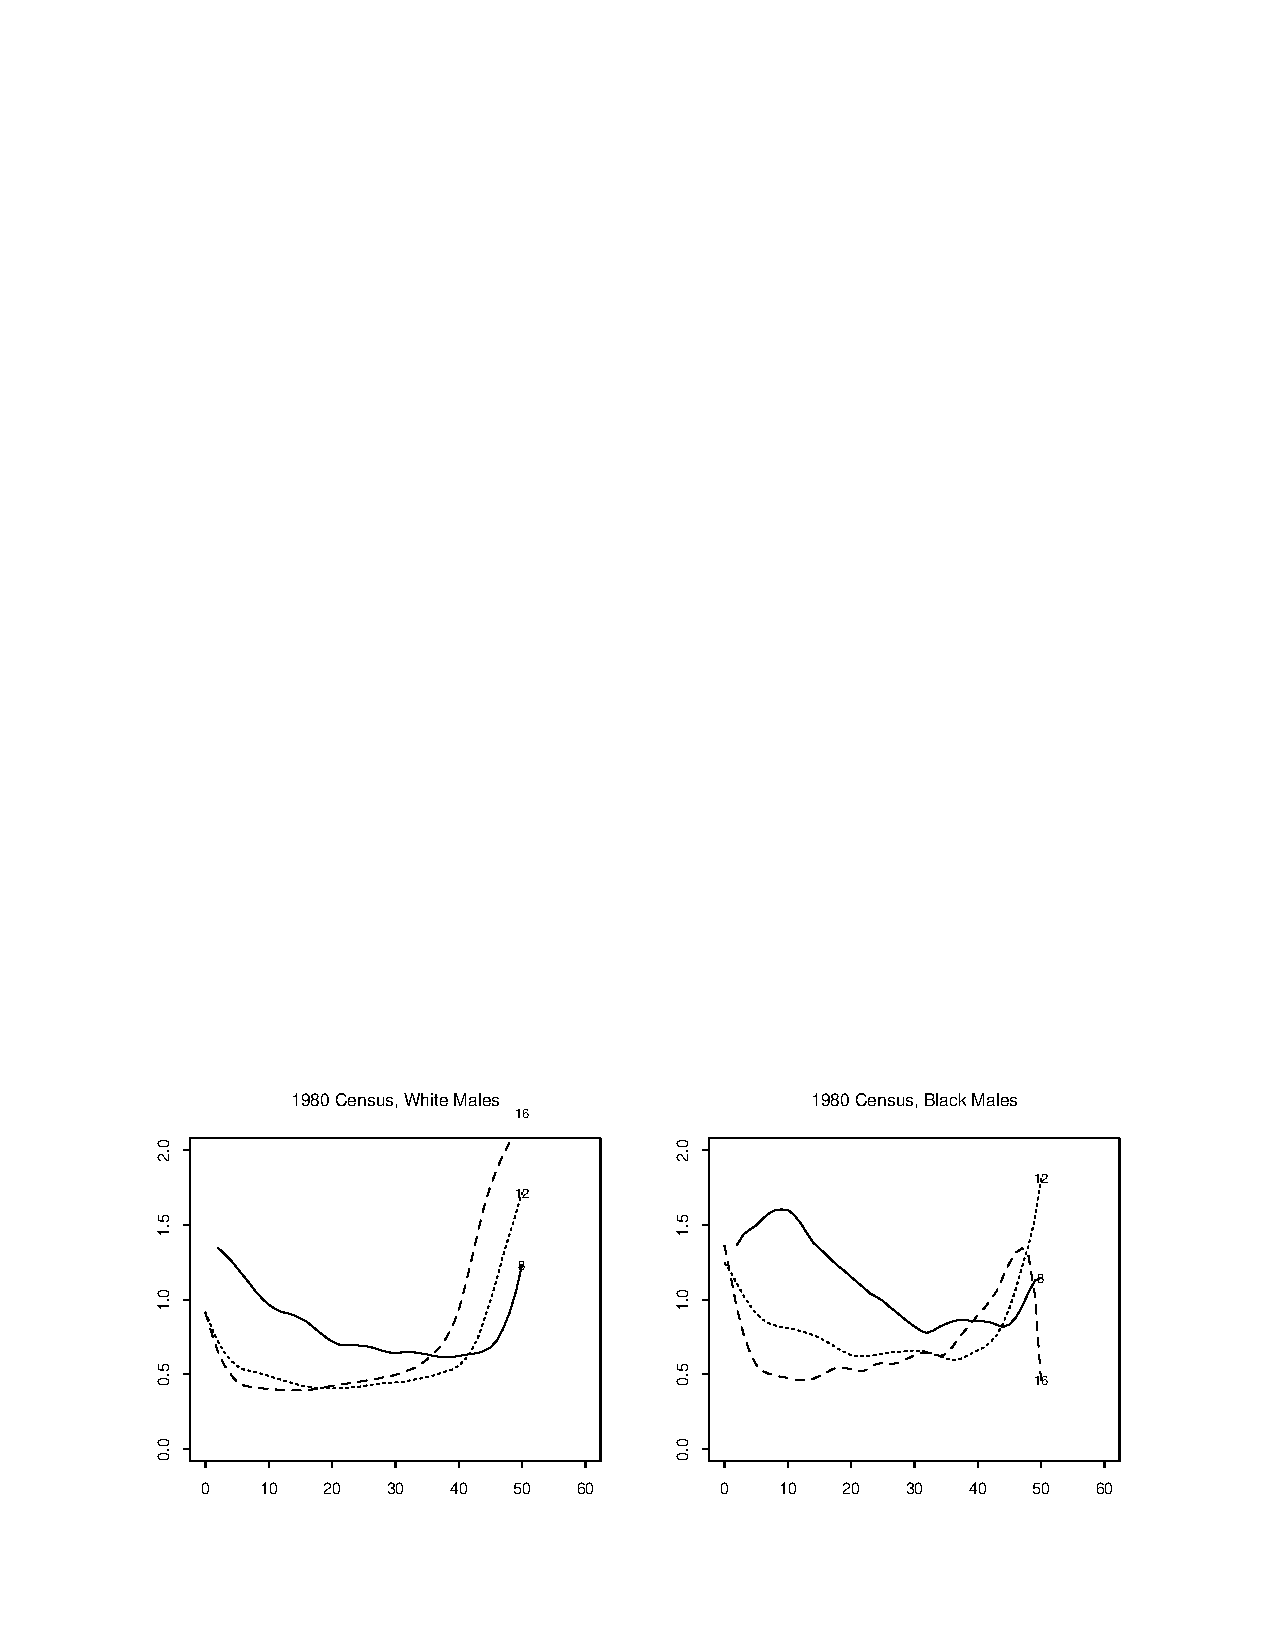
\includegraphics[width=.90\columnwidth]{fig-mincer-variance-1980}
\end{center}
\end{frame}
%-------------------------------------------------------------------------------
%-------------------------------------------------------------------------------
\begin{frame}
In the end, \citeA{Heckman.2006a} conclude:\vspace{0.5cm}

\begin{quote}
In common usage, the coefficient on schooling in a regression of log earnings on years of schooling is often called a rate of return. In fact, it is a price of schooling from a hedonic market wage equation. It is a growth rate of market earnings with years of schooling and not an internal rate of return measure, except under stringent conditions which we specify, test and reject in this chapter.
\end{quote}
\end{frame}
%-------------------------------------------------------------------------------
%-------------------------------------------------------------------------------
\begin{frame}[plain]
\begin{center}
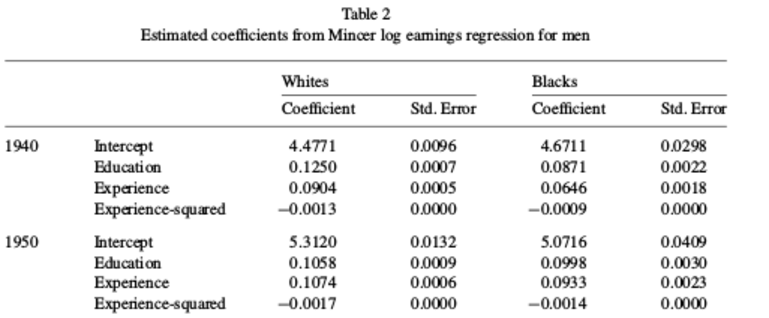
\includegraphics[width=.90\columnwidth]{tab-mincer-returns}
\end{center}
\end{frame}
%-------------------------------------------------------------------------------
%-------------------------------------------------------------------------------
